\documentclass{article}
\usepackage[utf8]{inputenc}
\usepackage{polski}
\usepackage{graphicx}
\usepackage{listings} 

\title{Sprawozdanie CSS}
\author{Jan Bronicki 249011\\Poniedziałek, 15:15 - 16:55 TN}
\date{}


\begin{document}

\maketitle

\begin{center}
    Kod jest dostępny na GitHubie:
    
\end{center}

\section{Wstęp}
Kaskadowe arkusze stylów (ang. Cascading Style Sheets, w skrócie CSS) – język służący do opisu formy prezentacji (wyświetlania) stron WWW. CSS został opracowany przez organizację W3C w 1996 r. jako potomek języka DSSSL przeznaczony do używania w połączeniu z SGML-em. Pierwszy szkic CSS zaproponował w 1994 r. Håkon Wium Lie.

Arkusz stylów CSS to lista dyrektyw (tzw. reguł) ustalających w jaki sposób ma zostać wyświetlana przez przeglądarkę internetową zawartość wybranego elementu (lub elementów) (X)HTML lub XML. Można w ten sposób opisać wszystkie pojęcia odpowiedzialne za prezentację elementów dokumentów internetowych, takie jak rodzina czcionek, kolor tekstu, marginesy, odstęp międzywierszowy lub nawet pozycja danego elementu względem innych elementów bądź okna przeglądarki. Wykorzystanie arkuszy stylów daje znacznie większe możliwości pozycjonowania elementów na stronie, niż oferuje sam (X)HTML.

CSS został stworzony w celu odseparowania struktury dokumentu od formy jego prezentacji. Separacja ta zwiększa zakres dostępności witryny, zmniejsza zawiłość dokumentu, ułatwia wprowadzanie zmian w strukturze dokumentu. CSS ułatwia także zmiany w renderowaniu strony w zależności od obsługiwanego medium (ekran, palmtop, dokument w druku, czytnik ekranowy). Stosowanie zewnętrznych arkuszy CSS daje możliwość zmiany wyglądu wielu stron naraz bez ingerowania w sam kod (X)HTML, ponieważ arkusze mogą być wspólne dla wielu dokumentów.
\section{Pierwsza strona CSS}


\begin{figure}[h!]
    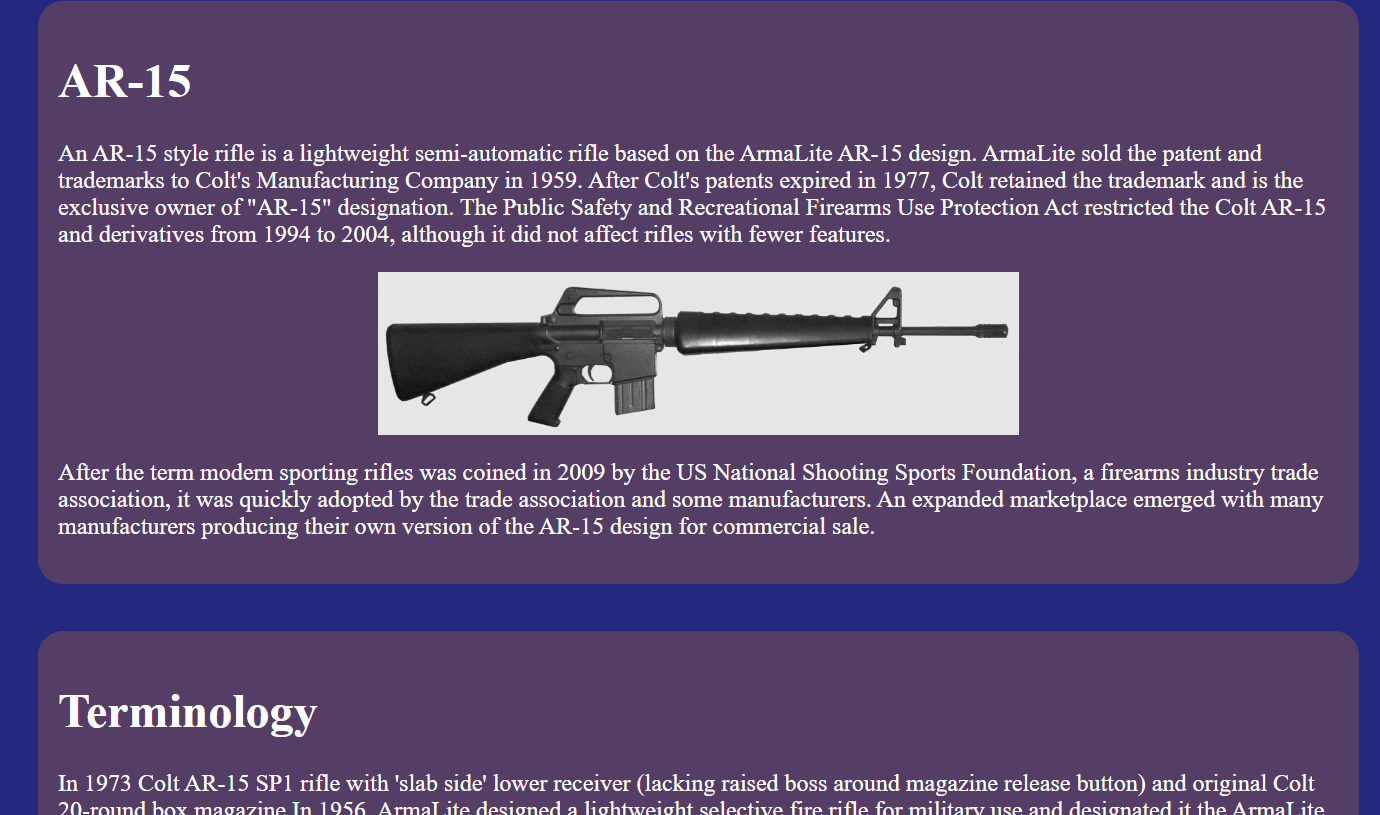
\includegraphics[scale=0.25]{1.png}
    \centering
\end{figure}


\begin{figure}[h!]
    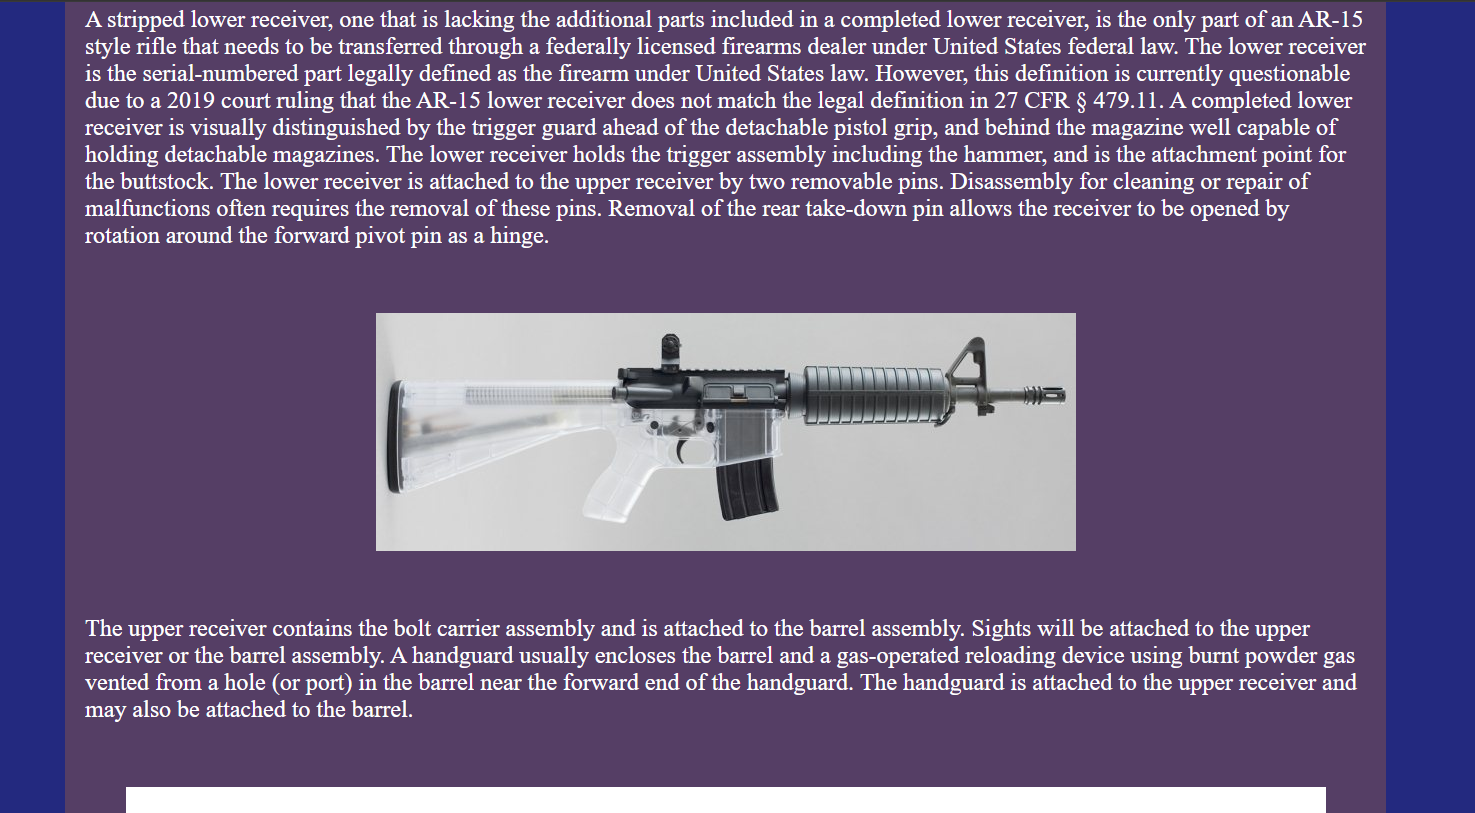
\includegraphics[scale=0.25]{2.png}
    \centering
\end{figure}
 
\newpage
\section{Druga strona CSS}

\begin{figure}[h!]
    
\includegraphics[scale=0.25]{3.png}
    \centering
\end{figure}







\end{document}